% Chapter 1

\chapter{Lex \c{s}i Yacc} % Write in your own chapter title
\label{Capitolul3}
\lhead{Capitolul 3. \emph{Lex \c{s}i Yacc}} % Write in your own chapter title to set the page header

Lex este un generator de analizoare lexicale \c{s}i constituie unul dintre utilitarele standard ale sistemelor de operare Unix.

Programul \emph{lex} prime\c{s}te la intrare un fi\c{s}ier con\c{t}in\^{a}nd o specifica\c{t}ie a atomilor pe care urmeaz\u{a} s\u{a}-i recunoasc\u{a} analizorul generat, precum \c{s}i a ac\c{t}iunilor semantice de executat. Pe baza acestei specifica\c{t}ii se genereaz\u{a} un program C ce con\c{t}ine tabelele de analiz\u{a}, \^{i}mpreun\u{a} cu func\c{t}ia de analiz\u{a}, numit\u{a} \emph{yylex( )}. \^{I}n continuare se compileaz\u{a} programul ob\c{t}inut, rezult\^{a}nd astfel analizorul lexical executabil. 

Fi\c{s}ierul ce con\c{t}ine specifica\c{t}ia este un fi\c{s}ier text care poate avea orice nume acceptat de sistemul de operare. Se recomand\u{a} ca fi\c{s}ierul de specifica\c{t}ie s\u{a} aibe extensia \emph{.l}.

Programul C rezultat este memorat \^{i}ntr-un fi\c{s}ier denumit implicit lex.yy.c (utilizatorul poate solicita explicit un alt nume).  Efectuarea analizei lexicale asupra unui text surs\u{a} folosind analizorul generat de LEX este ilustrat\u{a} \^{i}n figura de mai jos.

\begin{figure}[htp]
 \centering
 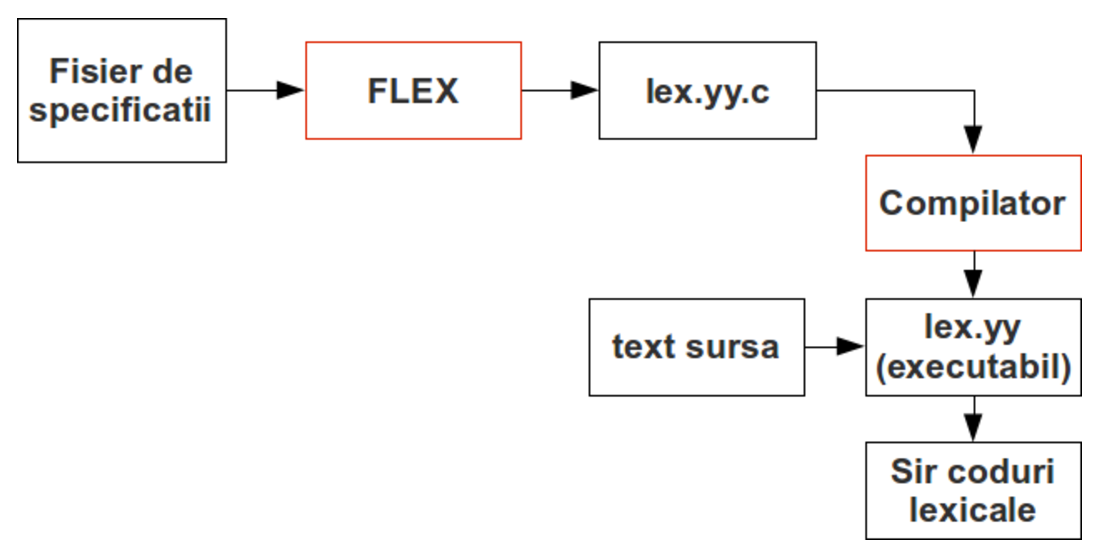
\includegraphics[scale=0.6]{Figuri/flex.eps}
 \caption{Analiza lexical\u{a} folosind Lex}
 \label{figflex}
\end{figure}

\section{Lansarea \^{i}n execu\c{t}ie a programului LEX}

Lansarea \^{i}n execu\c{t}ie a programului LEX se realizeaz\u{a} cu comanda
\begin{center}
lex [\emph{op\c{t}iuni}] [\emph{nume\_fi\c{s}ier\_specifica\c{t}ii}]
\end{center}
\^{I}n cazul \^{i}n care \emph{nume\_fi\c{s}ier\_specifica\c{t}ii} nu este precizat, LEX va a\c{s}tepta introducerea specifica\c{t}iilor de la stdin. 

C\^{a}teva dintre op\c{t}iunile liniei de comand\u{a} mai des utilizate sunt:
\begin{itemize}
	\item \emph{-d} = analizorul generat va func\c{t}iona \^{i}n regim "debug", adic\u{a} la fiecare atom recunoscut se va afi\c{s}a pe stderr un mesaj care con\c{t}ine num\u{a}rul liniei din fi\c{s}ierul de specifica\c{t}ii unde apare regula ata\c{s}at\u{a} atomului respectiv \c{s}i secven\c{t}a de caractere ce compun atomul; se precizeaz\u{a} c\u{a} efectul op\c{t}iunii \emph{-d} se ob\c{t}ine cu condi\c{t}ia ca variabila global\u{a} \emph{yy\_flex\_debug} s\u{a} fie setat\u{a} pe o valoare nenul\u{a}  (implicit variabila are valoarea 0);
	\item \emph{-h} = genereaz\u{a} la stdout un rezumat al op\c{t}iunilor din linia de comand\u{a} (-? \c{s}i --help au acela\c{s}i efect);
	\item \emph{-i} = analizorul generat va fi case-insensitiv (la identificatorii \c{s}i cuvintele cheie din textul surs\u{a} nu se va face distinc\c{t}ie \^{i}ntre literele mari \c{s}i cele mici);
	\item \emph{-o} = nume\_fi\c{s}ier\_ie\c{s}ire = aceast\u{a} op\c{t}iune se folose\c{s}te dac\u{a} se dore\c{s}te ca fi\c{s}ierul de ie\c{s}ire al generatorului s\u{a} aibe alt nume dec\^{a}t lex.yy.c;
	\item \emph{-T} = generatorul va lucra \^{i}n regim "trace", furniz\^{a}nd informa\c{t}ii utile care reflect\u{a} mersul procesului de construire a automatelor finite (nedeterminist \c{s}i determinist);
	\item \emph{-V} = la stdout se afi\c{s}eaz\u{a} versiunea programului LEX;
	\item \emph{-+} = analizorul generat va fi \^{i}n limbajul C++ (implicit el este \^{i}n ANSI-C).
\end{itemize}

Programul FLEX permite exprimarea unor op\c{t}iuni \c{s}i \^{i}n cadrul programului de specifica\c{t}ie \^{i}nsu\c{s}i, prin utilizarea directivei \emph{\%option} plasat\u{a} \^{i}n sec\c{t}iunea de defini\c{t}ii.

\section{Structura programului de specifica\c{t}ie}
Programul de specifica\c{t}ie con\c{t}ine \^{i}n principiu expresiile regulate ce descriu atomii limbajului surs\u{a}, precum \c{s}i ac\c{t}iunile pe care analizorul trebuie s\u{a} le execute la recunoa\c{s}terea fiec\u{a}rui atom.

Structura unui program de specifica\c{t}ie este urm\u{a}toarea:
\begin{verbatim}
sectiune definitii
%%
sectiune reguli
%%
cod utilizator
\end{verbatim}

\subsection{Sec\c{t}iunea de defini\c{t}ii}
Este utilizat\u{a} \^{i}n principal pentru a asocia nume expresiilor regulate, \^{i}n scopul ob\c{t}inerii unei specifica\c{t}ii mai simple \c{s}i mai clare.

\^{I}n afar\u{a} de aceasta, \^{i}n sec\c{t}iunea de defini\c{t}ii mai pot sa apar\u{a}:
\begin{itemize}
	\item directive \emph{\%option}
	\item declara\c{t}ii de st\u{a}ri de start
	\item secven\c{t}e C definite de utilizator
\end{itemize}
Pentru asocierea numelor cu expresiile regulate se utilizeaz\u{a} o construc\c{t}ie de forma:
\begin{center}
nume defini\c{t}ie
\end{center}
unde:
\begin{itemize}
	\item \textbf{nume} este un cuv\^{a}nt compus din una sau mai multe litere, cifre, '\_' sau '-', cu observa\c{t}ia c\u{a} primul caracter \emph{trebuie} s\u{a} fie liter\u{a} sau '\_' \c{s}i \emph{s\u{a} se afle pe prima pozi\c{t}ie a liniei};
	\item \textbf{defini\c{t}ie} este o expresie regulat\u{a} \c{s}i se consider\u{a} c\u{a} \^{i}ncepe cu primul caracter non-spa\c{t}iu de dup\u{a} nume \c{s}i \c{t}ine p\^{a}n\u{a} la sf\^{a}r\c{s}itul liniei.
\end{itemize}

Odat\u{a} declarat, un nume poate fi utilizat \^{i}n alte expresii regulate, sub forma:
\begin{center}
\{nume\}
\end{center}

Se poate considera c\u{a} numele asociate cu expresiile regulate sunt tratate \^{i}ntr-un mod similar directivelor \emph{\#define} dintr-un program C.

Directivele \emph{\%option} permit utilizatorului s\u{a} precizeze unele op\c{t}iuni legate de analizorul generat. C\^{a}teva asemenea op\c{t}iuni sunt:

\begin{itemize}
	\item \emph{\%option main} - are ca efect generarea unei func\c{t}ii main() care nu face altceva decat s\u{a} apeleze func\c{t}ia de analiz\u{a} yylex();
	\item \emph{\%option caseless} - are acela\c{s}i efect ca \c{s}i op\c{t}iunea -i din linia de comand\u{a};
	\item \emph{\%option debug} - are acela\c{s}i efect ca \c{s}i op\c{t}iunea -d din linia de comand\u{a}; 
	\item \emph{\%option yylineno} - analizorul rezultat va con\c{t}ine cod care actualizeaz\u{a} variabila global\u{a} yylineno cu valoarea curent\u{a} a num\u{a}rului liniei surs\u{a}; 
	\item \emph{\%option noyywrap} - aceast\u{a} op\c{t}iune este foarte util\u{a} dac\u{a} se dore\c{s}te ca la o rulare a analizorului s\u{a} se parcurg\u{a} un singur fi\c{s}ier surs\u{a}, a\c{s}a cum de fapt trebuie s\u{a} se \^{i}nt\^{a}mple de cele mai multe ori. 
\end{itemize}

Dac\u{a} aceast\u{a} op\c{t}iune lip\c{s}este, analizorul generat \^{i}ncearc\u{a} s\u{a} prelucreze \^{i}n lan\c{t} mai multe fi\c{s}iere surs\u{a}. Trecerea de la un fi\c{s}ier la altul se realizeaz\u{a} prin apelul de c\u{a}tre analizor a unei func\c{t}ii numite yywrap(), la \^{i}nt\^{a}lnirea marcajului EOF al fiec\u{a}rui fi\c{s}ier surs\u{a}. Cum func\c{t}ia yywrap() nu exist\u{a} \^{i}n mod implicit, ea ar trebui definit\u{a} de c\u{a}tre utilizator. Rolul acestei func\c{t}ii este s\u{a} deschid\u{a} urm\u{a}torul fi\c{s}ier \^{i}n variabila global\u{a} FILE *yyin \c{s}i s\u{a} returneze 0, respectiv s\u{a} returneze o valoare nenul\u{a} dac\u{a} nu mai exist\u{a} un fi\c{s}ier urm\u{a}tor.

Utilizatorul are posibilitatea de a plasa \^{i}n sec\c{t}iunea de defini\c{t}ii secven\c{t}e proprii de cod C. O modalitate de a introduce aceste secven\c{t}e C este ca ele s\u{a} fie incluse \^{i}ntre perechile de caractere \%\{ \c{s}i respectiv \%\}. Perechile \%\{ \c{s}i \%\} trebuie s\u{a} apar\u{a} pe linii separate \c{s}i neindentate. 

Codul cuprins \^{i}ntre aceste perechi (exclusiv perechile) va fi copiat ad-literam \^{i}n analizorul generat, \^{i}n spa\c{t}iul de vizibilitate din afara func\c{t}iei yylex(). Cu alte cuvinte, codul utilizator plasat \^{i}n sec\c{t}iunea de defini\c{t}ii va fi considerat ca spa\c{t}iu de declara\c{t}ii globale \^{i}n raport cu func\c{t}ia yylex().

\^{I}ntruc\^{a}t orice linie indentat\u{a} din sec\c{t}iunea de defini\c{t}ii este copiat\u{a} f\u{a}r\u{a} modific\u{a}ri \^{i}n analizorul generat, rezult\u{a} c\u{a} perechile delimitatoare \%\{ \c{s}i \%\} pot lipsi, cu condi\c{t}ia ca toate liniile de cod ale utilizatorului s\u{a} fie scrise indentat. 

\subsection{Sec\c{t}iunea de reguli}

Scopul principal al acestei sec\c{t}iuni este acela de a asocia ac\c{t}iuni semantice cu expresiile regulate. \^{I}n plus, ea mai poate con\c{t}ine cod C definit de utilizator.

Pentru asocierea ac\c{t}iunilor semantice cu expresiile regulate se utilizeaz\u{a} o construc\c{t}ie de forma:
\begin{center}
\c{s}ablon ac\c{t}iune
\end{center}
unde:
\begin{itemize}
	\item \textbf{\c{s}ablon} este o expresie regulat\u{a}, al c\u{a}rei prim caracter \emph{trebuie s\u{a} se afle pe prima pozi\c{t}ie a liniei};
	\item \textbf{ac\c{t}iune} este o secven\c{t}\u{a} format\u{a} din una sau mai multe instruc\c{t}iuni C care \emph{trebuie s\u{a} \^{i}nceap\u{a} pe aceea\c{s}i linie cu \c{s}ablonul}. Dac\u{a} secven\c{t}a e format\u{a} din mai multe instruc\c{t}iuni, acestea se vor \^{i}nchide \^{i}ntre acolade. \^{I}n particular, ac\c{t}iunea poate fi \c{s}i instruc\c{t}iunea vid\u{a}.
\end{itemize}

Semnifica\c{t}ia unei asemenea construc\c{t}ii este c\u{a} analizorul generat va executa secven\c{t}a descris\u{a} ca ac\c{t}iune atunci c\^{a}nd va recunoa\c{s}te \^{i}n textul surs\u{a} un \c{s}ir care se potrive\c{s}te cu \c{s}ablonul. 

Dac\u{a} ac\c{t}iunea este redat\u{a} prin instruc\c{t}iunea vid\u{a}, la recunoa\c{s}terea \c{s}irului descris de \c{s}ablonul \^{i}n cauz\u{a}, analizorul nu va executa nimic (de fapt, va trece pur \c{s}i simplu la delimitarea urm\u{a}torului atom). \^{I}n consecin\c{t}\u{a}, atomii ale c\u{a}ror reguli au ac\c{t}iune vid\u{a} sunt neglija\c{t}i (filtra\c{t}i sau elimina\c{t}i). Comentariile \c{s}i spa\c{t}iile albe sunt exemple de \c{s}iruri care se preteaz\u{a} la un asemenea tratament.

Dac\u{a} o ac\c{t}iune se termin\u{a} cu instruc\c{t}iunea return, aceasta va \^{i}nsemna ie\c{s}irea din func\c{t}ia yylex(), altfel aceast\u{a} func\c{t}ie trece automat la c\u{a}utarea urm\u{a}toarelor potriviri. \^{I}n concluzie, dac\u{a} dorim ca analizorul lexical s\u{a} prelucreze c\^{a}te un singur atom la fiecare apel, va trebui s\u{a} prevedem instruc\c{t}iuni return la toate ac\c{t}iunile care corespund unor atomi valizi (nu comentarii sau spa\c{t}ii albe). Acest mod de lucru este potrivit pentru compilatoarele care lucreaz\u{a} \^{i}ntr-o singur\u{a} trecere. Pentru compilatoarele care lucreaz\u{a} \^{i}n mai multe treceri, analiza lexical\u{a} fiind o faz\u{a} distinct\u{a}, ac\c{t}iunile se vor termina prin instruc\c{t}iuni de scriere (de exemplu directiva ECHO) a codurilor lexicale \^{i}ntr-un fi\c{s}ier de ie\c{s}ire (care ar putea fi yyout). 

\paragraph{Exemple de variabile utile:}
\begin{itemize}
	\item char *yytext - reprezint\u{a} adresa zonei de memorie \^{i}n care se depun caracterele ce compun atomul curent;
	\item int yyleng - reprezint\u{a} lungimea atomului curent;
	\item FILE *yyin - desemneaz\u{a} fi\c{s}ierul care con\c{t}ine textul surs\u{a} de analizat;
	\item FILE *yyout - desemneaz\u{a} fi\c{s}ierul \^{i}n care se poate scrie cu ajutorul macro-ului ECHO.
\end{itemize}

\paragraph{Exemple de macrouri \c{s}i func\c{t}ii utile:}
\begin{itemize}
	\item ECHO - realizeaz\u{a} scrierea con\c{t}inutului zonei yytext \^{i}n fi\c{s}ierul desemnat prin yyout;
	\item BEGIN nume\_stare\_start - realizeaz\u{a} comutarea analizorului \^{i}n starea de start specificat\u{a};
	\item REJECT - caut\u{a} urm\u{a}toarea regul\u{a} a c\u{a}rei \c{s}ablon se potrive\c{s}te cu atomul \^{i}n curs de prelucrare, sau cu un prefix al acestuia, \c{s}i execut\u{a} ac\c{t}iunea asociat\u{a} regulii g\u{a}site;
	\item YY\_START - furnizeaz\u{a} starea de start curent\u{a} (o valoare \^{i}ntreag\u{a});
	\item yyterminate() - are ca efect terminarea procesului de analiza \c{s}i returnarea valorii 0 c\u{a}tre apelantul func\c{t}iei yylex(); yyterminate() este un macro \c{s}i poate fi redefinit\u{a} de utilizator;
	\item void yymore() - determin\u{a} concatenarea urm\u{a}torului atom din textul surs\u{a} la atomul existent \^{i}n yytext (\^{i}n mod normal, urm\u{a}torul atom \^{i}l \^{i}nlocuie\c{s}te pe cel precedent);
	\item void yyless(int n) - las\u{a} \^{i}n yytext primele n caractere ale atomului curent, restituind \^{i}n \c{s}irul de intrare caracterele de pe pozi\c{t}iile n+1 p\^{a}n\u{a} la sf\^{a}r\c{s}it; actualizeaz\u{a} apoi valoarea lui yylen la n (caracterele restituite vor fi analizate ulterior);
	\item void unput(char c) - for\c{t}eaza plasarea \^{i}n \c{s}irul de intrare a caracterului c, acesta devenind urm\u{a}torul caracter de analizat;
	\item int input() - cite\c{s}te \c{s}i returneaz\u{a} urm\u{a}torul caracter din \c{s}irul de intrare.
\end{itemize}

\section{Expresii regulate}

Prima etap\u{a} \^{i}n \^{i}n\c{t}elegerea unui program este descompunerea lui \^{i}n lexeme. Se nume\c{s}te lexem\u{a}, un \c{s}ir de caractere de la intrare care este \^{i}n curs de analizare. 

De exemplu, \^{i}n C avem lexeme de forma for, while, etc., dar nu lexeme de forma \%\$\#@.

\^{I}n plus, \^{i}n C putem \^{i}nt\^{a}lni lexeme de genul variabila\_cea\_mare. Exist\u{a} deci un numar poten\c{t}ial infinit de lexeme (dac\u{a} presupunem c\u{a} numele de variabile nu au nicio limit\u{a} pentru lungime).

Teoreticienii au propus \^{i}n anii 1960 un meta-limbaj extrem de concis pentru a descrie lexeme. Limbajul acesta este limbajul expresiilor regulate. O expresie regulat\u{a} este un \c{s}ir de caractere care descrie o mul\c{t}ime de cuvinte posibile (poate chiar o mul\c{t}ime infinit\u{a}). Lexemele tuturor limbajelor de programare moderne pot fi descrise prin expresii regulate.

Pe baza expresiilor regulate se poate construi un automat cu st\u{a}ri finite, care st\u{a} la baza func\c{t}ionarii unui analizor lexical. Un automat cu st\u{a}ri finite este o ma\c{s}ina abstract\u{a} care poate analiza \c{s}i recunoa\c{s}te expresiile regulate, iar implementarea software a unui astfel de automat nu este dificil\u{a}.

Folosind expresiile regulate, se poate defini o gramatic\u{a} de expresii pentru un limbaj surs\u{a}.

Semnifica\c{t}ia expresiilor regulate:
\begin{itemize}
	\item . - semnific\u{a} orice caracter cu excep\c{t}ia lui newline;
	\item * - semnific\u{a} zero sau mai multe apari\c{t}ii ale expresiei regulate precedente;
	\item {[}{]} - semnific\u{a} o clas\u{a} de caractere;
	\item \^ - un circumflex la \^{i}nceputul unei expresii regulate semnific\u{a} faptul c\u{a} expresia respectiv\u{a} trebuie s\u{a} apar\u{a} chiar la \^{i}nceputul unei linii \^{i}n limbajul surs\u{a};
	\item \$ - un dolar la \^{i}nceputul unei expresii regulate semnific\u{a} faptul c\u{a} expresia respectiv\u{a} trebuie s\u{a} apar\u{a} chiar la sfar\c{s}itul unei linii \^{i}n limbajul surs\u{a};
	\item \{\} - indic\u{a} un domeniu restr\^{a}ns de copii ale expresiei regulate precedente. De exemplu, (abc)\{3,8\} semnific\u{a} \^{i}ntre 3 \c{s}i 8 apari\c{t}ii ale cuvantului 'abc';
	\item + - semnific\u{a} una sau mai multe apari\c{t}ii ale expresiei regulate precedente;
	\item ? - semnific\u{a} zero sau o singur\u{a} apari\c{t}ie a expresiei regulate precedente;
	\item \textbar - expresia regulat\u{a} precedent\u{a}, sau expresia regulat\u{a} urm\u{a}toare;
	\item "..." - tot ce este cuprins \^{i}ntre ghilimele se interpreteaz\u{a} literal;
	\item () - grupeaz\u{a} o serie de expresii regulate \^{i}ntr-o expresie nou\u{a}.
\end{itemize}

\section{Utilizarea generatorului de parsere Yacc}
Yacc poate genera un traducator \^{i}n modul urm\u{a}tor: specifica\c{t}iile sintactice precum \c{s}i unele elemente semantice sunt incluse \u{i}ntr-un fi\c{s}ier de intrare pentru Yacc. Acest fi\c{s}ier are \^{i}n general extensia ".y". Linia de comanda (in UNIX):
\begin{center}
yacc nume\_fisier.y
\end{center}
produce, plec\^{a}nd de la specifica\c{t}iile cuprinse \^{i}n fi\c{s}ierul de intrare nume\_fi\c{s}ier.y, un program scris \^{i}n limbaj C care implementeaz\u{a} metoda de analiz\u{a} sintactica LARL pentru gramatica respectiv\u{a} - \^{i}n spe\c{t}\u{a} func\c{t}ia yyparse(). Fi\c{s}ierul de intrare (programul surs\u{a}) pentru Yacc are structura urm\u{a}toare:
\begin{verbatim}
Declaratii
%%
Reguli
%%
Rutine C
\end{verbatim}

Partea Declara\c{t}ii a fi\c{s}ierului surs\u{a} este op\c{t}ional\u{a} \c{s}i poate cuprinde dou\u{a} sec\c{t}iuni. O prim\u{a} sec\c{t}iune cuprinde \^{i}ntre delimitatorii \%\{ \c{s}i \%\} declara\c{t}ii \^{i}n limbajul C pentru variabilele care se utilizeaz\u{a} \^{i}n regulile de traducere sau \^{i}n procedurile din cea de-a treia parte a fi\c{s}ierului. A\c{s}adar, textul cuprins \^{i}ntre \%\{ \c{s}i \%\} se copie nealterat \^{i}n fi\c{s}ierul C produs de Yacc. A doua sec\c{t}iune a acestei prime p\u{a}rti con\c{t}ine declara\c{t}ii ale unit\u{a}\c{t}ilor lexicale ale gramaticii, declara\c{t}ii de asociativitate \c{s}i preceden\c{t}\u{a} a operatorilor, declara\c{t}ii ale tipurilor de date pentru valorile semantice ale simbolurilor gramatacii.

Simbolurile terminale ale gramaticii,cu excep\c{t}ia celor formate dintr-un singur caracter (precum +, * etc), trebuiesc declarate. Aceste simboluri sunt reprezentate \^{i}n Yacc prin ni\c{s}te coduri numerice; func\c{t}ia yylex transmite codul unit\u{a}\c{t}ii respective func\c{t}iei yyparse. Programatorul nu trebuie s\u{a} \c{s}tie aceste coduri numerice, ele sunt generate automat folosind op\c{t}iunea -d la lansarea Yacc \c{s}i sunt trecute \^{i}ntr-un fi\c{s}ier nume.tab.h (sau yytab.h sub DOS). Unit\u{a}\c{t}ile lexicale se definesc prin linii de forma:
\begin{verbatim}
% token <nume_unitate_lexicala>
\end{verbatim}
\c{s}i pot fi utilizate \^{i}n celelalte dou\u{a} par\c{t}i ale fi\c{s}ierului de intrare. Tot \^{i}n aceast\u{a} sec\c{t}iune se poate introduce simbolul de start al gramaticii, \^{i}n cazul \^{i}n care aceasta nu este partea st\^{a}nga a primei reguli sintactice:
\begin{verbatim}
start <nume_simbol_de_start>
\end{verbatim}

Alte linii care pot fi incluse \^{i}n aceast\u{a} sec\c{t}iune sunt:
\begin{itemize}
	\item type - pentru definirea tipului;
	\item left - pentru asociativitate st\^{a}nga a operatorilor;
	\item right - pentru asociativitate dreapta a operatorilor;
	\item prec - pentru precizarea preceden\c{t}ei operatorilor;
	\item nonassoc - pentru declara\c{t}iile de neasociativitate.
\end{itemize}

Simbolurile gramaticii pot avea valori semantice. \^{I}n mod implicit, aceste valori sunt valori \^{i}ntregi \c{s}i sunt specificate \^{i}n YYSTYPE. Pentru a specifica alt tip, \^{i}n partea de declara\c{t}ii C se adaug\u{a} o directiv\u{a} define pentru YYSTYPE:
\begin{verbatim}
#define YYSTYPE <nume tip>
\end{verbatim}

Utilizarea de tipuri diferite pentru simboluri diferite se realizeaz\u{a} prin specificarea acestor tipuri \^{i}ntr-o declara\c{t}ie union (specific\u{a} Yacc) \c{s}i declararea tipului simbolurilor cu type. Iat\u{a} un exemplu:
\begin{verbatim}
%union {
	int intval;
	double doubleval;
	symrec *tptr;
}
type <intval> INT
type <doubleval> REAL
type <tptr> ID
\end{verbatim}

Prin aceste declara\c{t}ii se specific\u{a} tipul valorilor pentru token-urile INT, REAL, ID ca fiind respectiv int, double, pointer la symrec (pointer \^{i}n tabela de simboluri).

Partea a doua a fi\c{s}ierului de intrare, \emph{Reguli}, este partea obligatorie. Aici se specific\u{a} regulile gramaticii care descriu sintaxa pe care dorim s\u{a} o verificam cu acest analizor. Fiecare regul\u{a} con\c{t}ine:
\begin{itemize}
	\item partea st\^{a}ng\u{a};
	\item partea dreapt\u{a};
	\item partea de ac\c{t}iune.
\end{itemize}

Partea st\^{a}ng\u{a} trebuie s\u{a} con\c{t}in\u{a} un neterminal al gramaticii, iar partea dreapt\u{a} \c{s}irul format din terminali \c{s}i neterminali, corespunz\u{a}tor unei reguli. Cele dou\u{a} p\u{a}r\c{t}i sunt desp\u{a}r\c{t}ite prin ":". Partea de ac\c{t}iune, cuprins\u{a} \^{i}ntre \{ \c{s}i \}, con\c{t}ine un text scris \^{i}n limbajul C care va fi inclus \^{i}n analizor \c{s}i reprezint\u{a} opera\c{t}iile care se execut\u{a} atunci c\^{a}nd analizorul realizeaz\u{a} o reducere cu regula specificat\u{a}. O regul\u{a} se termin\u{a} prin ";". Dac\u{a} sunt mai multe reguli care au aceea\c{s}i parte st\^{a}nga, acestea se scriu o singura dat\u{a} \c{s}i par\c{t}ile drepte se despart prin "\textbar". Iat\u{a}, spre exemplu, cum se scriu regulile gramaticii care descrie expresiile aritmetice:
\begin{verbatim}
expr : NUMAR
| expr '+' expr
| expr '-' expr
| expr '*' expr
| expr '/' expr
| '(' expr ')'
;
\end{verbatim}

Aici, expr este numele neterminalului care define\c{s}te expresia aritmetic\u{a}, terminalii +, -, *, /, (, ) se pun \^{i}ntre apostrof, iar NUMAR reprezint\u{a} token-ul num\u{a}r. Dac\u{a} dorim ca analizorul pe care \^{i}l contruim s\u{a} realizeze \c{s}i ac\c{t}iuni semantice, de pild\u{a} s\u{a} evalueze expresiile, se adug\u{a} la reguli partea de ac\c{t}iune:
\begin{verbatim}
expr : NUMAR {$$ = $1;}
| expr '+' expr {$$ = $1+$3;}
| expr '-' expr {$$ = $1-$3;}
| '(' expr ')' {$$ = $2;}
;
\end{verbatim}

\^{I}n partea de ac\c{t}iune se scriu instruc\c{t}iuni \^{i}n limbajul C. Aici, \$\$ reprezint\u{a} valoarea unui atribut al neterminalului expr din st\^{a}nga regulii sintactice, iar \$i reprezint\u{a} valoarea atributului celui de-al i-lea simbol din partea st\^{a}nga a reguluii.

Ultima parte a fi\c{s}ierului de intrare con\c{t}ine rutine scrise \^{i}n limbaj C care se includ nealterate \^{i}n analizorul ob\c{t}inut de Yacc. \^{I}n aceast\u{a} parte trebuie furnizat un analizor lexical, adic\u{a} o func\c{t}ie yylex() precum \c{s}i apelul la func\c{t}ia yyparse() pe care o creeaz\u{a} Yacc.

\section{YACC: Recursivitatea \c{s}i ambiguitatea}
La specificarea unei liste, acest lucru se poate face fie folosind recursivitatea st\^{a}nga:
\begin{verbatim}
list : list ',' item { ... }
 | item { ... }
\end{verbatim}
fie folosind recursivitatea dreapta:
\begin{verbatim}
list : item ',' list { ... }
 | item { ... }
\end{verbatim}

Dac\u{a} folosim recursivitatea dreapta, toate elementele din list\u{a} sunt puse \^{i}n stiv\u{a}. Dup\u{a} ce ultimul item este introdus, abia atunci se \^{i}ncepe reducerea acestora. \^{I}n cazul recursivit\u{a}\c{t}ii st\^{a}nga, niciodat\u{a} nu vom avea mai mult de trei elemente \^{i}n stiv\u{a}, deoarece la fiecare trei se poate realiza o reducere, pe m\u{a}sur\u{a} ce ace\c{s}tia sunt furniza\c{t}i de scanner. Din acest motiv, este recomandat\u{a} folosirea recursivit\u{a}\c{t}ii st\^{a}nga.

Un conflict ce apare frecvent este acela al construc\c{t}iilor de tip if-then-else. S\u{a} consider\u{a}m c\u{a} avem urm\u{a}toarele produc\c{t}ii:

\begin{verbatim}
stmt : IF expr THEN stmt
 | IF expr THEN stmt ELSE stmt
 ...
\end{verbatim}
\c{s}i urm\u{a}torul context (unde am marcat cu . locul unde am ajuns cu parcurgerea instruc\c{t}iunii curente):

\begin{verbatim}
IF expr THEN stmt IF expr THEN stmt . ELSE stmt
\end{verbatim}

Trebuie s\u{a} decidem dac\u{a} shift\u{a}m ELSE sau reducem contextul IF expr THEN stmt care se afl\u{a} deja pe v\^{a}rful stivei. Limbajele de programare precizeaz\u{a} c\u{a} ELSE apar\c{t}ine celui mai inferior IF, deci trebuie \^{i}n acest caz s\u{a} realiz\u{a}m un shift. Aceast\u{a} ambiguitate se rezolv\u{a} acord\^{a}nd construc\c{t}iei if-then-else o preceden\c{t}\u{a} mai mare dec\^{a}t celei simple if-then:

\begin{verbatim}
%nonassoc IF_SIMPLU
%nonassoc ELSE

stmt : IF expr THEN stmt %prec IF_SIMPLU
 | IF expr THEN stmt ELSE stmt
\end{verbatim}

Acela\c{s}i tip de construc\c{t}ie se utilizeaz\u{a} \c{s}i la definirea preceden\c{t}ei produc\c{t}iei ata\c{s}ate minusului unar, de exemplu.

\section{Exemplu lex si yacc}
S\u{a} lu\u{a}m ca exemplu realizarea unui parser care s\u{a} recunoasc\u{a} toate \c{s}irurile limbajului:
\begin{equation}
 L=\left \{ w \mid w = a^{n}b^{n}, n\geqslant 0 \right \}
\end{equation} 
Gramatica acestui limbaj este:
\begin{verbatim}
A -> a A b | ab
\end{verbatim}

unde A este unicul neterminal \c{s}i \^{i}n acela\c{s}i timp simbol de start iar terminalii (tokenii) gramaticii sunt a \c{s}i b.

Vom scrie mai \^{i}nt\^{a}i scannerul ce recunoa\c{s}te tokenii limbajului dat. Acesta este urm\u{a}torul:
\begin{verbatim}
%{
#include "ex1.tab.h"
%}

%%

a	{return TOKEN_A;}
b	{return TOKEN_B;}
\.	{return yytext[0];}
.	{printf("tokenul %s nu este cunoscut\n", yytext);}
\n	{return yytext[0];}

%%
\end{verbatim}

Sec\c{t}iunea de defini\c{t}ii include fi\c{s}ierul ex1.tab.h ce va fi generat de yacc \c{s}i con\c{t}ine declara\c{t}iile tokenilor limbajului (TOKEN\_A \c{s}i TOKEN\_B).

Prima regul\u{a} din sec\c{t}iunea a doua specific\u{a} faptul c\u{a} fiecare apari\c{t}ie a caracterului "a" \^{i}n textul surs\u{a} reprezint\u{a} TOKEN\_A. La fel pentru cea de-a doua, care se refer\u{a} la "b". Cea de-a treia recunoa\c{s}te punctul. La \^{i}nt\^{a}lnirea lui, scannerul il recunoa\c{s}te \c{s}i \^{i}l paseaz\u{a} parser-ului ca atare, f\u{a}r\u{a} a-i asocia vreun cod. Cea de-a patra regul\u{a} se potrive\c{s}te tuturor celorlalte caractere recunoscute la intrare, iar ac\c{t}iunea asociat\u{a} afi\c{s}eaz\u{a} un mesaj de eroare. Aceasta nu se termin\u{a} cu "return", astfel scannerul p\u{a}streaza mai departe controlul - adic\u{a} tokenul recunoscut de aceast\u{a} regul\u{a} este ignorat de parser. \^{I}n fine, ultima regul\u{a} recunoa\c{s}te caracterul "newline" \c{s}i \^{i}l transmite ca atare parserului.

Sec\c{t}iunea de subrutine nu con\c{t}ine nimic \^{i}n cazul specific\u{a}rii scannerului.

Regulile gramaticii sunt precizate de fi\c{s}ierul ex1.y. Parserul are o procesare orientat\u{a} pe linii. Vom mai \^{i}mbog\u{a}\c{t}i gramatica astfel:

\begin{verbatim}
%token TOKEN_A TOKEN_B

%%

S : S T '\n'	{printf("n = %d\n", $2);}
 | S '\n'		{ /* linie goala testata */ }
 | S '.'		{return;}
 |				/* regula implicita */
 ;

T : TOKEN_A T TOKEN_B	{ $$ = $2 + 1; }
 | TOKEN_A TOKEN_B		{ $$ = 1; }
 ;
 
%%

int main(void)
{
	yyparse();
	return 0;
}

int yyerror(char *s)
{
	printf("%s\n", s);
}
\end{verbatim}

Prima sec\c{t}iune con\c{t}ine defini\c{t}iile tokenilor. Cea de-a doua descrie gramatica, ce are \^{i}n cazul ales \c{s}ase produc\c{t}ii. Simbolul de start este S. Deoarece el are o produc\c{t}ie lambda, aceasta este redus\u{a} implicit, adic\u{a} f\u{a}r\u{a} a citi nimic de la intrare, parserul \^{i}l va plasa pe S pe varful stivei. Pentru prima produc\c{t}ie a lui S, se detecteaz\u{a} o linie complet\u{a} ce con\c{t}ine un cuvant din limbajul specificat, deci se poate afi\c{s}a n. \$2 indic\u{a} valoarea celui de-al doilea neterminal din partea dreapt\u{a}, care este T, adic\u{a} un cuv\^{a}nt al limbajului. A doua produc\c{t}ie a lui S precizeaz\u{a} ac\c{t}iunea de realizat atunci c\^{a}nd se introduce o linie vid\u{a} (dac\u{a} se introduce "newline" \c{s}i pe stiv\u{a} nu era decat S, atunci acest neterminal se pastreaz\u{a}). A treia produc\c{t}ie pentru S va executa "return" din analizorul sintactic atunci c\^{a}nd utilizatorul introduce caracterul punct, adic\u{a} procesarea se \^{i}ncheie.

Produc\c{t}iile pentru T sunt relativ familiare. Ac\c{t}iunile de urmat sunt \^{i}ns\u{a} interesante. Astfel, pentru a doua produc\c{t}ie a lui T, se detecteaz\u{a} un nucleu ab, iar valoarea asociat\u{a} neterminalului rezultat al reducerii acestui \c{s}ir este 1. Prima regul\u{a} recunoa\c{s}te recursiv \c{s}iruri de dimensiuni din ce \^{i}n ce mai mari, iar valoarea neterminalului la care se reduce contextul recunoscut se calculeaz\u{a} prin incrementarea valorii neterminalului \^{i}ncadrat \^{i}ntre un a \c{s}i un b ce constituie handle-ul.

Sec\c{t}iunea de subrutine define\c{s}te func\c{t}ia main precum \c{s}i func\c{t}ia yyparse de tratare a erorilor de sintax\u{a}.
